\chapter{Other contributions}

\section{Acoustic Novelty Detection with Adversarial Autoencoders}
\begin{figure}[h]
	\begin{subfigure}[t]{0.9\columnwidth}
		\def\svgwidth{0.5\columnwidth}
		% This file was created by matlab2tikz.
%
%The latest updates can be retrieved from
%  http://www.mathworks.com/matlabcentral/fileexchange/22022-matlab2tikz-matlab2tikz
%where you can also make suggestions and rate matlab2tikz.
%


\begin{tikzpicture}

\begin{axis}[%
width=0.85\columnwidth,
height=4cm,
at={(1.424in,0.703in)},
scale only axis,
point meta min=-156.535576728001,
point meta max=-22.4028070325664,
axis on top,
xmin=0.008,
xmax=29.992,
ytick={0,1,...,8},
x label style={at={(axis description cs:0.50,-0.06)},anchor=north},
y label style={at={(axis description cs:0.0,0.4)},anchor=south},
xlabel style={font=\color{white!15!black}},
xlabel={Time (s)},
ymin=-0.015625,
ymax=8.015625,
ylabel style={font=\color{white!15!black}},
ylabel={Frequency (kHz)},
axis background/.style={fill=white},
colormap/jet
%colorbar,
%colorbar style={ylabel style={font=\color{white!15!black}}, ylabel={Power/frequency (dB/Hz)}}
]
\addplot [forget plot] graphics [xmin=0.008, xmax=29.992, ymin=-0.015625, ymax=8.015625] {img/spectrogram-1_highlight.png};
%\draw[black,line width=2pt] (axis cs:4.7,4) ellipse (12 and 400);

%\draw[line width=1.2pt](axis cs:3.65,8) rectangle (axis cs:5.7,0);

%\node [draw, ellipse, thick, red, minimum width=14, minimum height=200, label=above:Novelty] at (axis cs:4.7,4) {};
\node[text=white] at (axis cs:4.7,4)[rotate=90] {\contour{white}{Novelty}};

%\draw[black,line width=2pt] (axis cs:18.5,4) ellipse (12 and 400);
%\draw[line width=1.2pt](axis cs:17.5,8) rectangle (axis cs:19.55,0);
\node[text=white] at (axis cs:11.6,4)[rotate=90] {\contour{white}{Novelty}};

%\draw[black,line width=2pt] (axis cs:25,0.5) ellipse (50 and 40);
%\draw[line width=1.2pt](axis cs:20,5) rectangle (axis cs:29.95,0);

%\fill[black, opacity=0.4](axis cs:20,5) rectangle (axis cs:29.95,0);
%\fill[white, opacity=0.5](axis cs:22,3) rectangle (axis cs:28.00,1);

\node[text=white] at (axis cs:25,4) {\contour{white}{Normal}};



\end{axis}
\end{tikzpicture}%
	\end{subfigure}	
	\caption[Acoustic Novelty Detection]{Spectrogram of an audio signal with novel and normal data.}
\end{figure}
Novelty detection is the task of recognising events the differ from a model of normality. This paper proposes an acoustic novelty detector based on neural networks trained with an adversarial training strategy. The proposed approach is composed of a feature extraction stage that calculates Log-Mel spectral features from the input signal. Then, an autoencoder network, trained on a corpus of ``normal'' acoustic signals, is employed to detect whether a segment contains an abnormal event or not. A novelty is detected if the Euclidean distance between the input and the output of the autoencoder exceeds a certain threshold. The innovative contribution of the proposed approach resides in the training procedure of the autoencoder network: instead of using the conventional training procedure that minimises only the Minimum Mean Squared Error loss function, here we adopt an adversarial strategy, where a discriminator network is trained to distinguish between the output of the autoencoder and data sampled from the training corpus. The autoencoder, then, is trained also by using the binary cross-entropy loss calculated at the output of the discriminator network.  

The performance of the algorithm has been assessed on a corpus derived from the PASCAL CHiME dataset. The results showed that the proposed approach provides an F1-score equal to 93.28\%, with a relative performance improvement equal to 0.26\% compared to the standard autoencoder. The significance of the improvement has been evaluated with a one-tailed z-test and resulted significant with $p<0.001$. The presented approach thus showed promising results on this task and it could be extended as a general training strategy for autoencoders if confirmed by additional experiments.

\subsection{Details}
In this work, we are not interested in the generative capabilities of the network, since in the novelty detection task the objective is to minimise the error made by the autoencoder in reconstructing normal data. Thus, the architecture and the training strategy are different from \cite{makhzani2015adversarial}: the discriminator network is trained to discriminate between data from a training set and data reconstructed by the autoencoder (\figref{fig:our_training}). The final layer of the discriminator is a single neuron with sigmoid activation function and its output represents the probability of the data of being sampled from the training set. At the end of the training phase, the discriminator network should not be able to distinguish training set data and reconstructed data, i.e., its output should be constantly equal to 0.5.

Similarly to \cite{goodfellow2014generative}, the training process can be viewed as a min-max game between the autoencoder and the discriminator network. Let $\boldsymbol{x}$ be an input feature vector, $\tilde{\boldsymbol{x}} = A(\boldsymbol{x})$ the output of the autoencoder, and $D(\boldsymbol{x})$ the output of the discriminator network, i.e., the probability of $\boldsymbol{x}$ of being sampled from the training data. The training procedure is composed of three main phases: the first phase and the third phase consist in updating the autoencoder and the discriminator respectively by minimising the reconstruction error and the classification error (binary cross-entropy). The middle phase incorporates the interaction between the two networks: the autoencoder weights are updated based on the output the discriminator network.


Whether a feature vector is a novel sound or a normal background sound is determined by calculating the reconstruction error, i.e., the Euclidean distance between the output produced by the autoencoder and the input data itself. If the distance exceeds a predefined threshold, the input data is classified as novelty, otherwise as normal. The threshold is calculated as follows: for each input sequence the threshold $\theta$ is calculated with the following expression:
\begin{equation}
\theta = \beta \cdot \text{median}\{e(1),\ldots,e(N)\},
\end{equation}
where $e(i)$ is reconstruction error of feature vector $i$ in the signal, $N$ is the number of features, and $\beta \in [1, 2]$ is a predefined constant.

\begin{figure}[h]
	\centering
	\begin{subfigure}[t]{0.7\columnwidth}
		\def\svgwidth{\columnwidth}
		\input{7_other_contributions/img/our_approach.pdf_tex}
		
		\caption{Proposed architecture for training an autoencoder with an adversarial discriminator network.}\label{fig:our_training}
	\end{subfigure}
	\par\bigskip
	\begin{subfigure}[t]{0.7\columnwidth}
		\def\svgwidth{\columnwidth}
		\input{7_other_contributions/img/detection.pdf_tex}
		
		\caption{Novelty detection phase.}\label{fig:our_detect}
	\end{subfigure}
	\caption[Acoustic Novelty Detection with GANs]{The proposed approach for novelty detection with adversarial autoencoders. For the sake of simplicity, the feature extraction stage is not shown.}\label{fig:approach}
\end{figure}

\newpage
\section[Siamese Nets for Human-Fall Detection]{Few-shot Siamese Neural Networks employing Audio features for Human-Fall Detection}

Nowadays, the detection of human fall is a problem recognized by the entire scientific community. Methods that have good performance use human falls samples in the train set, while methods that do not use it, can only work well under certain conditions. Since examples of human falls are very difficult to retrieve, there is a strong need to develop systems that can work well event with few or no data to be used for their training phase. In this work, we show a first study on few-shot learning Siamese Neural Network applied to human falls detection by using audio signals. This method has been compared with algorithms based on SVM and OCSVM, all evaluated starting from the same conditions. The proposed approach is able to learn the differences between signals belonging to different classes of events. In classification phase, using only one human fall signal as a template, it achieves about 80\% of  $ F_1 -Measure$ related to the human fall class, while the SVM based method gets around 69\%, when it is trained in the same data knowledge conditions.

\subsection{Proposed Approach}

In this work we propose a Siamese Neural Network able to learn a latent representation of an audio event. In particular, a SNN is composed of two twin networks with binded weights. A pair of inputs is provided to the system, one to each twin network. Downstream, the network maps these inputs into two different representation vectors. Then, a certain type of distance between those two representations is computed. In this work euclidean distance was used. In \figref{proposed_approach}, are reported two example of mel-spectrograms: the spectrum that is given as input to the function first network represents a chair that is overturned. The other inputs instead represent a human fall. As can be seen, the signals are not distinguishable at a glance, thus we think that the differential approach of the SNN, described below, seems to be appropriate.

Our Siamese network has been trained on a corpus of labelled object fall events and not including any human fall. Pairs of events belonging to the same class correspond to the positive examples while pairs of events belonging to the different class a negative one. In particular, the term few-shot comes from the fact that although, in this case study, human falls have not been used for training, some of them are used in the optimization phase, before the final test.
\begin{figure}
	\centering
	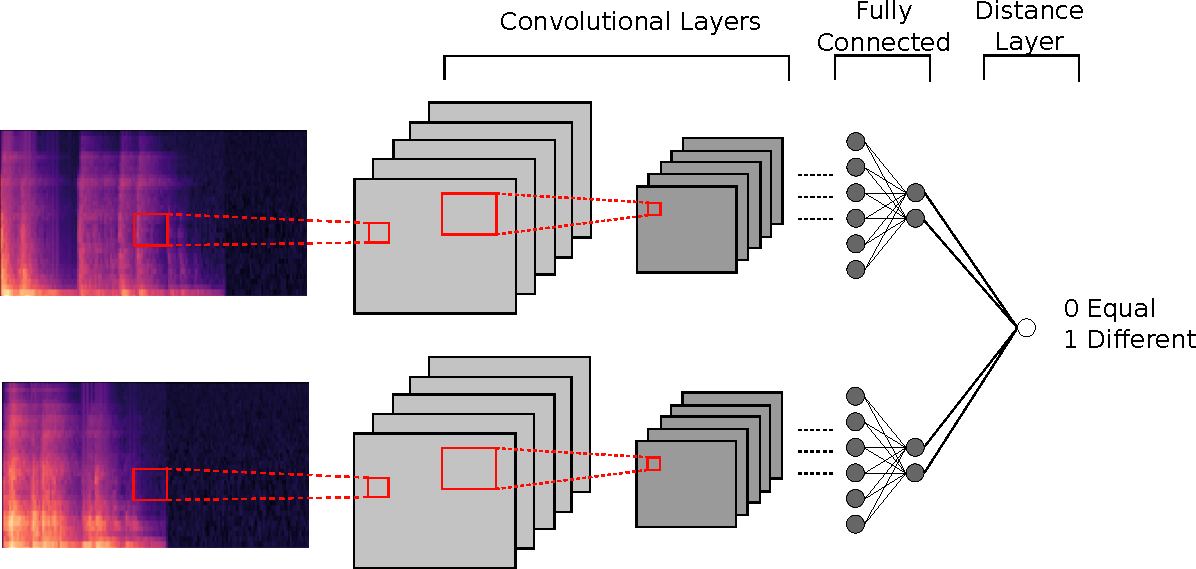
\includegraphics[width=0.7\linewidth]{img/Siamese_approach}
	\caption[Siamese Nets for Human-Fall Detection]{Proposed approach for Human-Fall Detection.}
	\label{proposed_approach}
\end{figure}

\subsection{Results}
The results obtained for each method are reported in \figref{fig:results_f1}. The figure shows the $ F_1 -Measure$, false negative rate (miss rate) and false positive rate (false alarm rate) referred to the human fall class. It is clear that the supervised SVM method outperforms all other in terms of  $ F_1 -Measure$ as expected. The OCSVM instead is the worst method if used in this context, because its training procedure does not include any human fall, but the normality model is composed of others types of falls, making it difficult to identify the human fall as ``novelty''. The Siamese and the SVM-unbalanced, which start from the same data for the training, are classified in the intermediate positions as expected. However, we note that the proposed approach achieves a better result, exceeding the $ F_1 -Measure$ of SVM-unbalanced of about 11\%. 

\begin{figure}[h]
	\centering
	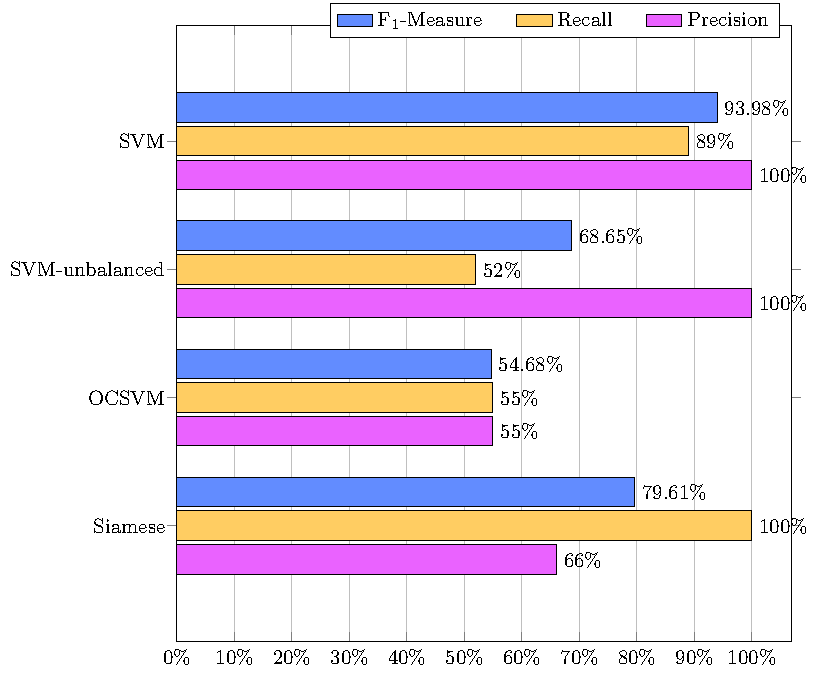
\includegraphics[width=0.65\linewidth]{img/results_f1}
	\caption[Siamese Nets for Human-Fall Detection - Results]{$F_1 -Measure$, precision and recall: the metrics are referred to the human fall class}
	\label{fig:results_f1}
\end{figure}


\newpage
%%%%%%%%%%%%%%%%%%%%%%%%%%%%%%%%%%%%%%%%%%%%%%%%%%%%%%%%%%%%%%%%%%%%%%%%%%%%%%%%%%%%%%%%%%%%%%%%%%%%%%%%%%

\section{Generative Raw Audio Synthesis}
Biologically-inspired algorithms such as artificial neural networks have been used extensively by computer music researchers, for generative music and algorithmic composition. The recent introduction of raw audio Machine Learning (ML) techniques, however, represents a significant leap because they seem to be able to learn both high-level (event) and low-level (timbre) information at once. Employing such techniques for creative purposes is very challenging at this early stage since there is lack of method, experience, and their computational cost is very high. 

To the best of our knowledge, three main architectures have been proposed to learn and reproduce features from raw audio signals, namely WaveNet \cite{van2016wavenet}, sampleRNN \cite{mehri2016samplernn}, and WaveGan \cite{donahue2018synthesizing}. Recently, another architecture, named FFTnet, has been proposed \cite{jin2018fftnet} that draws some concepts from WaveNet but shows a lower computational cost. 

These architectures show the ability of learning features from raw audio data and generate similar signals drawing from a \textit{latent} representation of these data directly in the time domain. This seems to be possible thanks to a hierarchical representation of the signal. In other words, architectures such as sampleRNN and WaveNet process the signal at multiple levels, enabling the network to store significant features from the micro-scale (sample level) up to the macro-scale (1 second and more). Experiments with these two architectures show that after training the network with a few hours of piano music, the networks are able to reproduce piano tones in a somewhat organized way. They are, thus, able to learn the timbre of the piano, the piano tone envelope (attack and decay), and finally, they learn that piano notes have rhythmical patterns, can be played in clusters, chords and sequences.

Stemming from these results, the authors decided to explore the possibility of running these algorithms for tone generation. At the time of writing, these algorithms are not suitable for synthesis from a score. However, they have the autonomous ability of generating a sequence of sounds, similarly to generative algorithms, but working at several time scales.

\subsection{Algorithm Selection}\label{subsec:algorithm}

A careful evaluation of currently available machine learning algorithms for raw-audio generation has been carried on. The evaluated algorithms were:
\begin{itemize}
	\item WaveNet \cite{van2016wavenet},
	\item sampleRNN \cite{mehri2016samplernn},
	\item WaveGAN \cite{donahue2018synthesizing}.
\end{itemize}

At the time of setting up the experiments the FFTNet algorithm \cite{jin2018fftnet} was not yet published.

The WaveNet architecture allows for modeling complex data such as music and speech. It is based on a stack of causal dilated convolutional layers for feature extraction. The dilated convolutions are key to extract features at different levels (closely resemblant to a dyadic wavelet filter bank \cite{jin2018fftnet}), however, the experiments in \cite{cabello2017autoregressive} show that the use of dilated convolutions alone do not allow modelling complex raw audio sequences, thus, residual blocks and the use of skip connections after the convolutional layers are necessary to speed up convergence and allow the training of a deep model. The ability of the network to model meaningful sequences of samples relies on causal probability conditioning, i.e. the last output sample is conditioned by the probability of all previous output samples. Additionally, it has been shown with speech synthesis that the output sample probability can be conditioned with, e.g. speaker timbre and phonemes. In our case, however, we are not interested in leveraging this feature, leaving the network to generate freely.

The main issue preventing adoption of WaveNet is its high computational cost and informal reports of their performance seems to confirm this. To test the feasibility of the approach and verify these claims we adapted one of the several open-source implementations of WaveNet currently available. We conducted preliminary experiments on a Titan X GPU employing Theano as backend. After 72 hours of training using the same piano dataset suggested by \cite{van2016wavenet} the network was still unable to provide results vaguely similar to the ones shown by the authors of \cite{van2016wavenet}. Furthermore, some of the hyperparameters were extrapolated from the paper, but most of them are not available, so a hyperparameters search would be required, increasing the training times far over our available resources.

A very different approach is followed by the authors of sampleRNN \cite{mehri2016samplernn}. This architecture is based on the same principle of causal probability conditioning, however, in this case the network consists of several tiers of recurrent neural networks (RNN) working at different temporal resolutions. Each RNN conditions the RNN at the lower tier. SampleRNN has been tested with both speech and music database. Both database are a few hours long.

We also performed preliminary experiments employing the open-source implementation provided by the authors of \cite{mehri2016samplernn} on the same hardware reported above. This implementation is based on Theano and Lasagne. Results are on par with those provided by the authors and training times can have length of 1-4 days depending on the input material and the degree of fitness that is required.

Finally, we considered WaveGAN for sound generation. This architecture is based on the generative adversarial networks (GAN) paradigm. The authors of \cite{donahue2018synthesizing} devised two models, WaveGAN, working on the raw audio with 1D convolutions and SpecGAN, working with 2D spectrograms. The outcomes of their work are very promising, since these two architecture are able to learn from a much shorter database than WaveNet and sampleRNN. However, they are inherently designed to synthesized audio of a specific length (16384 samples for WaveGAN or a 128x128 spectrogram for SpecGAN). For this reason they are not well suited for generative audio. Running a WaveGAN several times would introduce issues in concatenating each output.

At the end of this evaluation stage, we decided to use sampleRNN. 


\subsection{Input Material and Dataset Creation}\label{subsec:input}

The input material for this work has been provided by artist \textit{\O kapi} in form of \textit{stems} of his musical project Rima Glottidis. The main goal of the work was to generate vocal textures from his material to be arranged in form of a site-specific sound installation. The stems came from cut recordings of male and female speech of several speakers showing proper Italian pronunciation vs. unclear spelling and regional accent.

Additionally they presented bell tones, singing choirs, sung phonemes, and silence, revealing part of the musical structure of the original project. The whole material length was 14 minutes. A subset of this material, totalling 7 minutes, was obtained by leaving only the speaking voices and cutting all other musical material.

From previous experience with sampleRNN the input material was judged to be too short. Informal experiments on voice synthesis were conducted in 2016 by the first author showing that sampleRNN can faithfully learn the vocal timbre of a speaker only from a sufficiently large and homogeneous dataset of speech. Specifically, a 3 hours dataset gathered from publicly available speeches of a well known Italian comedian and politician was used to train a three-tier sampleRNN model. At the end of the training, a convincing babbling was obtained with random phonemes. Most subjects presented with the synthesized speech could recognize the identity of the public figure. Reducing the dimension of the dataset to 1 hour or less degraded the performance of the network making the utterances noise-like.

To increase the chances to obtain interesting audio material from sampleRNN, other audio material has been selected. Data augmentation has been tested to enlarge the training corpus without adding spurious material that would reduce the portion of material from \textit{\O kapi}. Data augmentation has been done by pitch shifting audio data by -3 and +3 semitones. 

Additionally, 22 minutes of choral works from Arvo P\"art were added. A subset of this dataset has been randomly selected, totalling 2 minutes. These datasets have been used for training 2 different sampleRNN models with hyperparameters suggested by the authors of \cite{mehri2016samplernn}. Training of these models was conducted with a Titan X GPU and left running for 2 days for each one, approximately lasting for 220 epochs (approx $3 \cdot 10^6$ iterations). For each epoch, several 10s-long pieces of randomly generated material were extracted for later use. 

\subsection{Results}
Discussion about the network outcomes will be qualitative, as there is no objective means to assess the quality of the material. The loss employed by sampleRNN, the categorical crossentropy, does not clearly state the quality of the sound material. The largest excursion of the loss seen during training ranged from 5 to 3 for the training set and from 4.5 to 3.9 for the validation set. Notwithstanding this, the first tones generated were pure noise, while the last ones had some of the character of the original dataset. The training loss did not necessarily decrease with time and samples with interesting features emerged at different epochs. Most notably, samples generated at a given epoch or at consecutive epochs, have all very similar features that later disappear with the training.

The outcomes from these trainings can be divided in several classes: speech-like babbling (a), whistling (b), rumbles and impulses (c) or mixtures of the above. Figure \ref{fig:esempi} shows spectrograms of each class. Please note that the whistling tones do not appear in the output generated from the Rima Glottidis speech-only subset. It was noted, indeed, that these have the same frequency of bell tones found in the complete Rima Glottidis dataset. Bell tones appear on the 5\% of the Rima Glottidis dataset. This means that very simple and repetitive material can be easily reproduced by sampleRNN even though it does appear on a small portion of the dataset.
\begin{figure}[h]
	\centering
	%\vspace{-0.5cm}
	
	\begin{subfigure}[b]{0.45\columnwidth}
		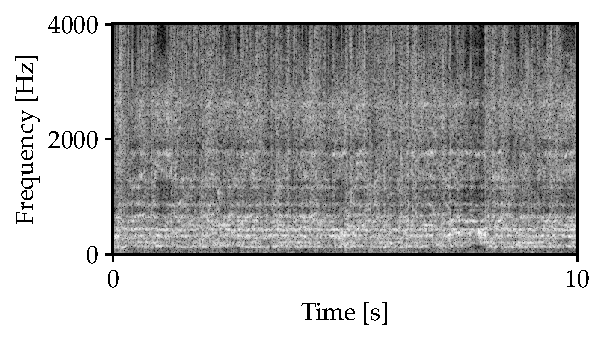
\includegraphics[width=\textwidth]{img/choral.pdf}
		\subcaption{}
	\end{subfigure}	
	\begin{subfigure}[b]{0.45\columnwidth}
		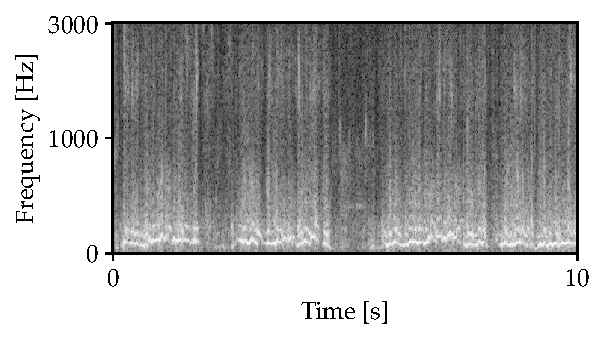
\includegraphics[width=\textwidth]{img/speech2.pdf}
		\subcaption{}
	\end{subfigure}
	
	\begin{subfigure}[b]{0.45\columnwidth}
		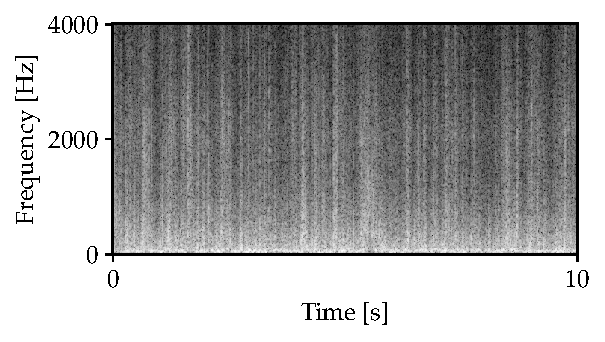
\includegraphics[width=\textwidth]{img/rumble.pdf}
		\subcaption{}
	\end{subfigure}	
	\begin{subfigure}[b]{0.45\columnwidth}
		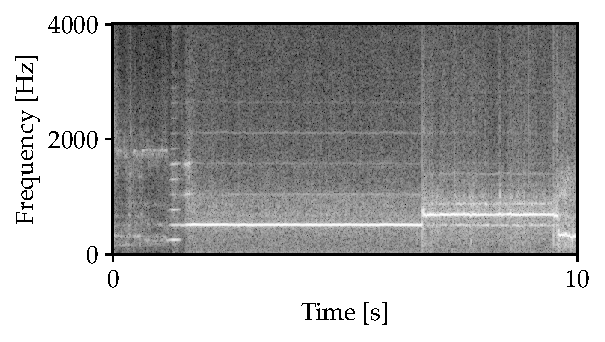
\includegraphics[width=\textwidth]{img/whistle.pdf}
		\subcaption{}
	\end{subfigure}
	
	
	\caption[SampleRNN - Raw Audio Generation]{Spectrograms of several classes of outputs from sampleRNN: choir textures (a), speech-like babbling (b), rumble (c), whistle (d). The choir textures are obtained from the Chorales training set, while the others are from the Rima Glottidis training set. The main two tones in Figure (d) are a C5 and a F5.}
	\label{fig:esempi}
\end{figure}